\chapter{DataBase NoSQL}
I database \emph{NoSQL}, che sta per \emph{not only SQL}, sono database non tabellari che archiviano i dati
in maniera completamente differente dai classici relazionali.
Le caratteristiche principali sono la progettazione specifica per carichi elevati e il supporto nativo per la scalabilitá
orizzontale, la tolleranza agli errori e la memorizzazione dei dati in modo denormalizzato.
Infatti ogni elemento viene archiviato singolarmente con una chiave univoca, e la coerenza dei dati non viene garantita.
Questa impostazione fornisce un approccio molto piú flessibile alla memorizzazione dei dati rispetto a un database
relazionale, un controllo migliore e una maggiore semplicitá nelle applicazioni.

\section{Perche é nato \emph{NoSQL}?}
A partire dagli anni 2000 si é passati da un modello in cui le persone principali dell'IT erano sistemisti ad un modello
in cui le persone principali sono diventate gli sviluppatori. Tale passaggio ha comportato la nascita di database NoSQL
che sono fortemente orientati agli sviluppatori ed allo sviluppo Agile.
Inoltre i dati si sono trasformati passando dai classici strutturati a dati non strutturati (di differenti dimensioni,
semistrutturati, polimorfici..) che non permettevano di definire un modello relazionale organico e cosí i database NoSQL sono
diventati estremamente popolari perché permettono di lavorare principalmente con dati non strutturati anche di enormi
dimensioni.

\section{Perché dovrei utilizzare un database \emph{NoSQL}?}
I database NoSQL sono una soluzione ideale per molte applicazioni moderne, quali dispositivi mobili, Web e videogiochi
che richiedono strutture dati flessibili, scalabili, con prestazioni elevate ed altamente funzionali.
\begin{itemize}
    \item \texttt{Flessibilitá}: vengono offerti schemi flessibile che consentono uno sviluppo piú veloce. Quindi é una soluzione ideale
    per i dati semi-strutturati e non strutturati. É possibile arricchire le applicazioni di nuovi dati e informazioni
    senza dover sottostare ad una rigida struttura dei dati;
    \item \texttt{Scalabilitá}: grazie alla semplicitá vi é la possibilitá di \emph{scalare in orizzontale} in maniera estremamente
    efficiente. Infatti, si predilige l'utilizzo di cluster con molti nodi distribuiti, rispetto all'utilizzo di server centralizzati.
    Inoltre, vi é la possibilitá di aggiungere nodi a caldo in maniera completamente trasparente per l'utente finale;
    \item \texttt{Elevate Prestazioni}: grazie alla mancanza di operazioni di aggregazione dei dati("join") ed anche grazie
    all'introduzione di semplificazioni, come il mancato supporto delle transazioni ACID, si ha una elevata velocitá computazionale.
    \item \texttt{Altamente funzionali}: non vi é piú un linguaggio generale (SQL) come nei database relazionali, ma vi sono
    API in base al database specifico che si va ad utilizzare.
\end{itemize}


\section{Tipologie di \emph{NoSQL}}
Tipologie principali di database \emph{NoSQL}:
\begin{itemize}
    \item \texttt{documentali}: la rappresentazione dei dati é affidata a strutture simili ad oggetti, dette \emph{documenti}, ognuno dei
    quali possiede un certo numero di proprietá che rappresentano le informazioni.
    Viene creata una semplice coppia, a una chiave viene assegnato un documento specifico, e in questo documento, il quale puó essere
    formattato in vari modi (XML, JSON, YAML ...) si possono trovare le informazioni.
    La nozione di schema é dinamica, ogni documento puó contenere appunto dei campi diversi. Questa flessibilitá puó essere particolarmente
    utile per la modellazione dei dati in cui le strutture possono cambiare da un record all'altro, ad esempio nei dati polimorfici.
    Inoltre, diventa piú semplice l'evoluzione di un'applicazione durante il suo ciclo di vita, ad esempio nel caso in cui vadano aggiunti nuovi
    campi.

    Tra gli esempi di maggiore interesse vi sono: MongoDB, Azure CosmosDB, Apache CouchDB.

    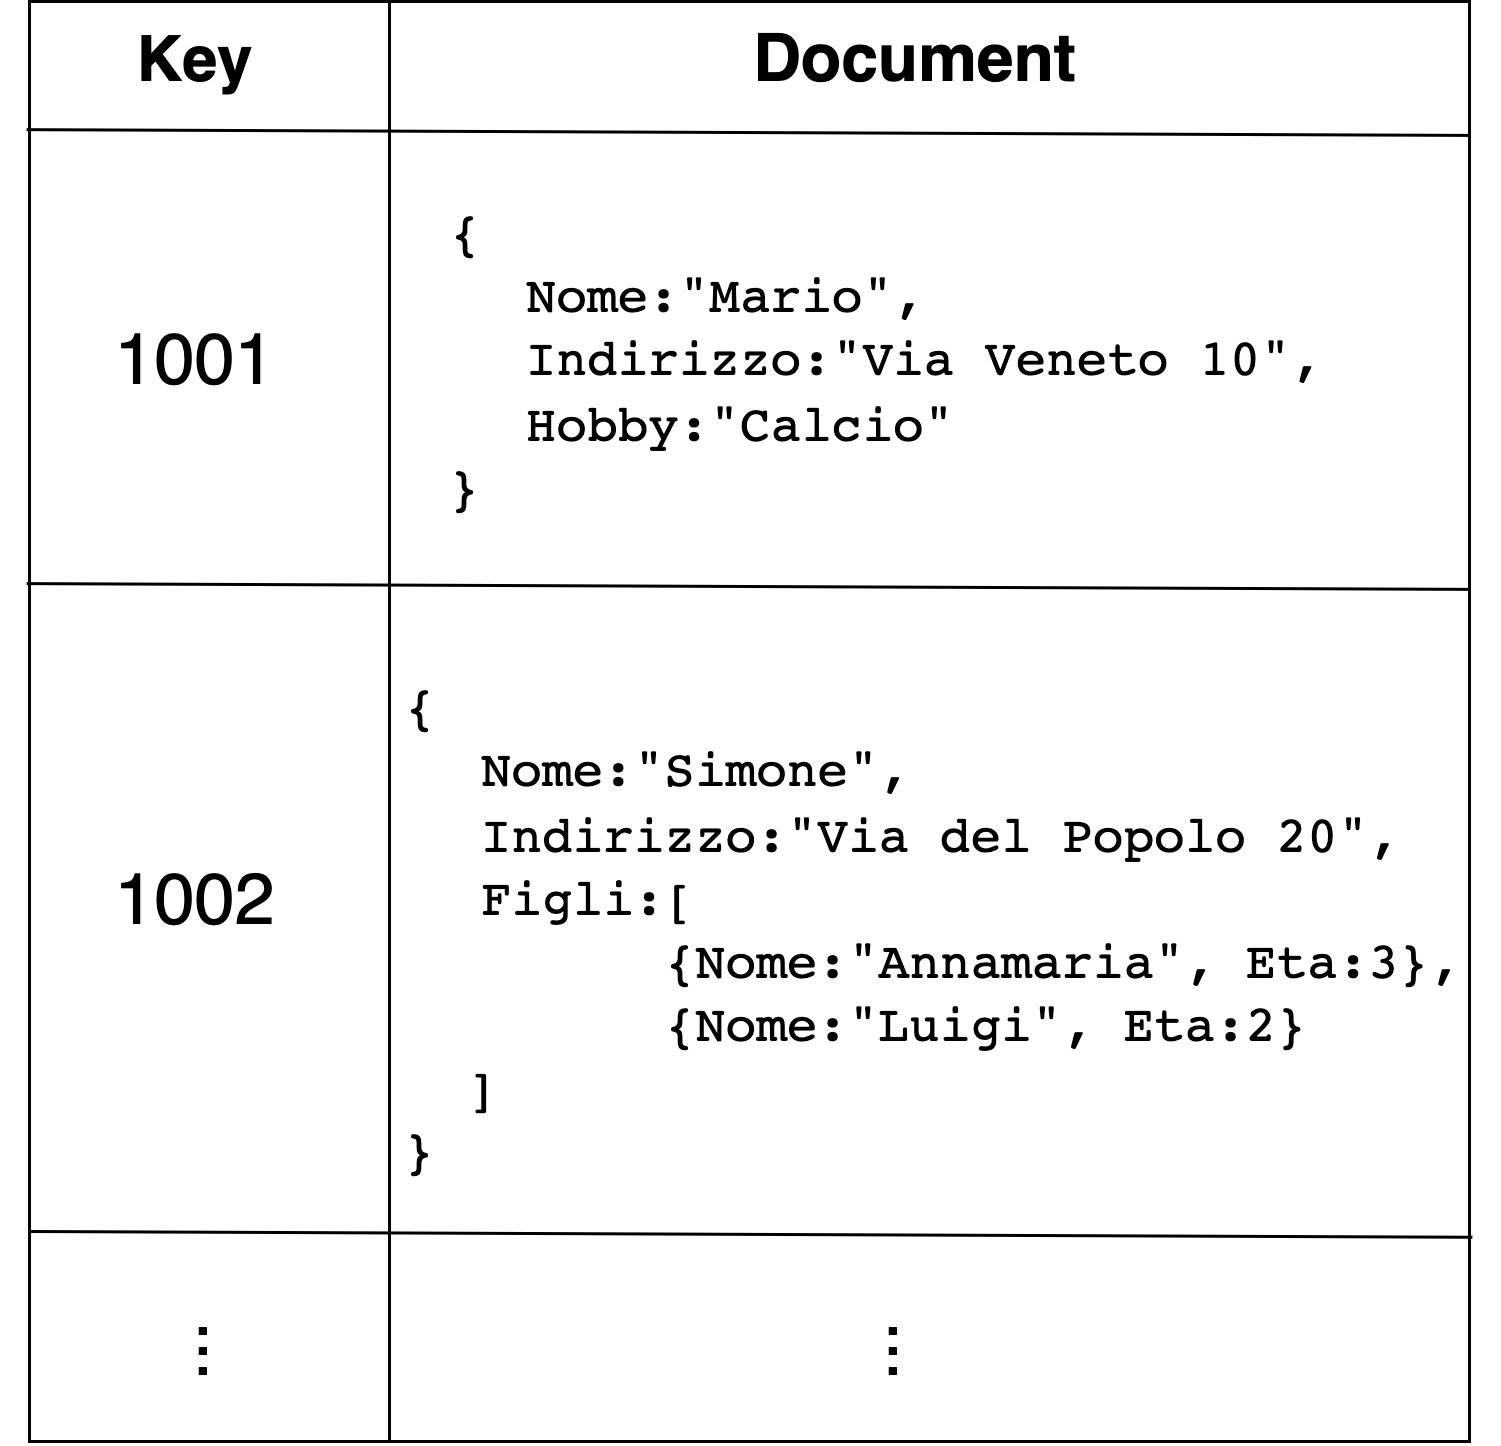
\includegraphics[width=1\textwidth]{img/dbDocumentale}

    \item \texttt{key-value}: i dati vengono immagazzinati mediante un semplice metodo chiave-valore. Una chiave rappresenta un identificatore
    univoco. Le chiavi e i valori possono essere qualsiasi cosa, da un oggetto semplice ad articolati oggetti composti.
    (Questo tipo di base di dati é oggetto di tesi e quindi verrá sviluppato il suo concetto nel corso dei prossimi capitoli.)

    Tra gli esempi di maggiore interesse vi sono: \textbf{Redis}, MemCached.
    \item \texttt{colonnari}: i dati vengono archiviati per colonne, anziché per righe come avviene nei database relazionali classici.
    Queste colonne vengono raccolte per formare dei sottogruppi. Le chiavi e i nomi delle colonne di questo tipo di database non sono fissi.
    Ogni colonna é memorizzata separatamente. Se sono presenti colonne simili, vengono unite in famiglie di colonne ed ogni famiglia
    viene archiviata separatamente dalle altre su un "file" diverso.
    Questa tipologia di database viene utilizzata quando é necessario un modello di dati di grandi dimensioni. Estremamente utili
    per i data warehouse, oppure quando sono necessarie prestazioni elevate o la gestione di query intensive.

    Tra gli esempi di maggiore interesse vi sono: HBase, Cassandra, Vertica.

    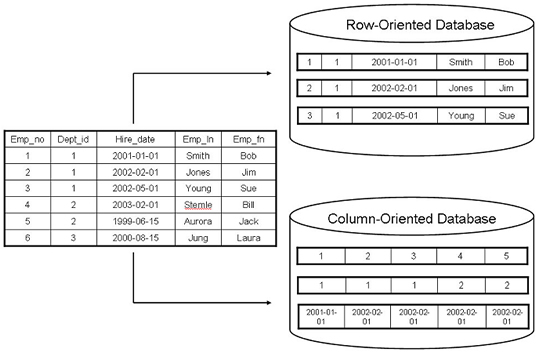
\includegraphics[width=0.8\textwidth]{img/dbColumnOriented}

    \item \texttt{a grafo}: progettati appositamente per l'archiviazione e la navigazione di relazioni. Le relazioni rivestono un ruolo chiave
    e buona parte del valore di questi database deriva proprio dalla loro presenza. Vengono utilizzati i \emph{nodi} per archiviare le entitá
    di dati e gli \emph{archi} per archiviare le relazioni tra entitá. Le relazioni che un nodo puó avere sono illimitate.
    In questo tipo di database attraversare collegamenti o relazioni é molto veloce perché le relazioni tra i nodi non vengono elaborate al momento
    della query, ma sono giá presenti nel database.
    I casi d'uso piú tipici sono i Social Network, motori di raccomandazioni e rilevamento di frodi, ovvero in tutti quegli ambiti dove é
    necessario creare molte relazioni tra dati ed eseguire rapidamente query su di esse.

    Tra gli esempi di maggiore interesse vi sono: Neo4J, Titan.

    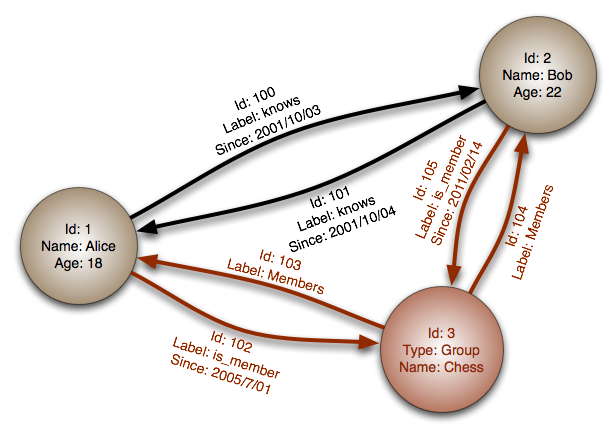
\includegraphics[width=0.8\textwidth]{img/dbGrafo}
\end{itemize}
